
    \section{Simple Geometry}
    This section will have alot of functions used in geometry problems. They are related to points, lines, circles and polygons.
    \subsection{Points, Lines and Polygons}
    This is the base of all codes in geometry. u can change the type from ldb to ll and also change the EPS. The rest is pretty much fixed.
    \inputwithhash{./solutions/Geometry/geobase.cpp}
    \subsection{Circles}
    This section will have alot of algorithms related to circles and their description.

    A tangent to a circle is a line in the plane of a circle which intersects the circle in exactly one point. This point is called the point of tangency.

    A tangent of two circles is a common internal tangent if the intersection of the tangent and the line segment joining the centers is not empty.

    \begin{center}
    \begin{minipage}{.5\textwidth}
    \centering
    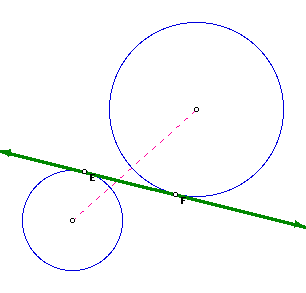
\includegraphics[scale = 0.5]{imgs/internal1.png}
    \end{minipage}%
    \begin{minipage}{0.5\textwidth}
    \centering
    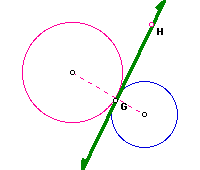
\includegraphics[scale = 0.5]{imgs/internal2.png}
    \end{minipage}
    \end{center}
    
    
    A tangent of two circles is a common external tangent if the intersection of the tangent and the line segment joining the centers is empty.

    
    \begin{center}
    \begin{minipage}{.5\textwidth}
    \centering
    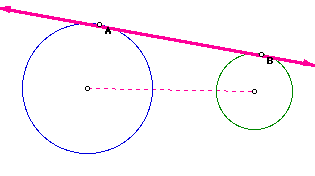
\includegraphics[scale = 0.5]{imgs/external1.png}
    \end{minipage}%
    \begin{minipage}{0.5\textwidth}
    \centering
    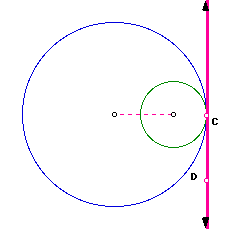
\includegraphics[scale = 0.5]{imgs/external2.png}
    \end{minipage}
    \end{center}

    The CircumCenter of a triangle is the minimum enclosing circle of a triangle. We can also calculated the minimum enclosing circle of a polygon.

    \begin{center}
    \begin{minipage}{.3\textwidth}
    \centering
    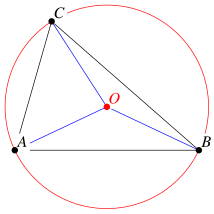
\includegraphics{imgs/circumcenter.png}
    \end{minipage}%
    \begin{minipage}{0.7\textwidth}
    \centering
    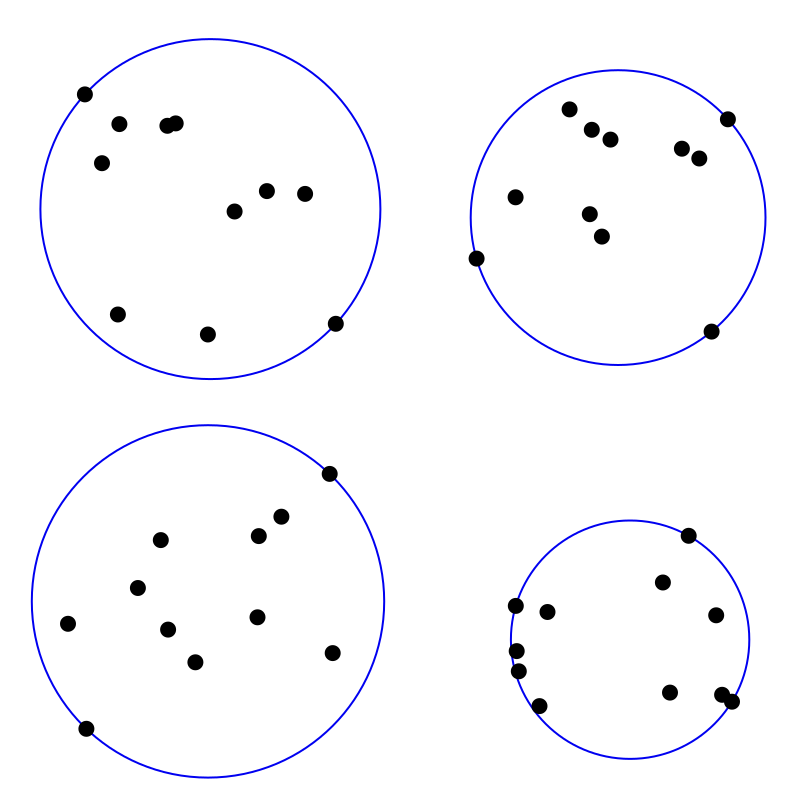
\includegraphics[scale = 0.5]{imgs/mec.png}
    \end{minipage}
    \end{center}

    \inputwithhash{./solutions/Geometry/circle.cpp}
